\chapter{Sviluppo del modulo nfproxy}

Il regex filtering è un modello di filtraggio che garantisce ottime prestazioni (grazie all'elaborazione tramite linguaggi e librerie ottimizzati), ma presenta forti limitazioni nella flessibilità di analisi del traffico.

Questa rigidità è particolarmente rilevante nei CTF, dove la maggior parte dei servizi utilizza protocolli come HTTP, che spesso includono contenuti compressi o codificati (es. Base64, gzip), difficilmente analizzabili tramite regex.\\

A discapito di prestazioni inferiori, nfproxy introduce il vantaggio di scrivere filtri in \texttt{Python}\footcite{\url{http://python.org/}}{python}, linguaggio semplice e rapido per lo scripting, superando i limiti precedenti e offrendo:

\begin{itemize}
    \setlength{\itemsep}{4pt}
    \setlength{\parskip}{4pt}
    \item Massima libertà nell'implementazione delle logiche di filtraggio
    \item Prestazioni comunque elevate grazie a scelte architetturali mirate
    \item Supporto nativo a compressioni/encoding comuni, tramite il parsing del protocollo applicativo
\end{itemize}

\texttt{Nfproxy} non è un proxy tradizionale ma un modulo basato su
\texttt{nfqueue}\footcite{\url{https://netfilter.org/projects/libnetfilter_queue/}}{netfilter_queue},
che permette un controllo sul traffico paragonabile ad un proxy classico, ma con accesso diretto ai pacchetti a livello di rete (layer 3/4) e con un'intercettazione del traffico invisibile all'applicativo.

Va riportata l'esistenza di limitazioni nella modifica dei pacchetti, che tuttavia non rappresenta uno scenario d'uso necessario per la difesa del servizio.

Il sistema combina C++ per un gestione efficiente dei pacchetti e Python per eseguire il parsing dei protocolli applicativi.

Questo approccio ibrido permette di sfruttare al meglio le caratteristiche di entrambi i linguaggi, garantendo prestazioni elevate e flessibilità nello sviluppo.

I protocolli attualmente supportati includono:
\begin{itemize}
    \setlength{\itemsep}{4pt}
    \setlength{\parskip}{4pt}
    \item HTTP/1.1\footcite{RFC2616, Hypertext Transfer Protocol -- HTTP/1.1}{rfc2616} (con gestione compressione/encoding del body)
    \item Websocket\footcite{RFC6455, The WebSocket Protocol}{rfc6455} (con decodifica dei frame e supporto alle estensioni)
    \item TCP standard\footcite{RFC9293, Transmission Control Protocol (TCP)}{rfc9293} (con ricostruzione dello stream)
\end{itemize}

\section{Requisiti}

Di seguito gli obiettivi fondamentali del modulo:

\begin{itemize}
    \setlength{\itemsep}{4pt}
    \setlength{\parskip}{4pt}
    
    \item \textbf{Integrazione con Python}: Fornire un'interfaccia in Python per implementare le regole di filtraggio, con funzioni ottimizzate e sintassi intuitiva.
    
    \item \textbf{Analisi avanzata di HTTP/1.1 e WebSocket}: Interpretazione nativa dei pacchetti applicativi, con estrazione automatica dei dati decodificati/decompressi. Supporto integrato per:
    \texttt{gzip}\footcite{RFC1952, GZIP file format specification version 4.3}{rfc1952},
    \texttt{deflate}\footcite{RFC1951, DEFLATE Compressed Data Format Specification version 1.3}{rfc1951},
    \texttt{brotli}\footcite{RFC7932, Brotli Compressed Data Format}{rfc7932},
    \texttt{zstd}\footcite{RFC8478, Zstandard Compression and the application/zstd Media Type}{rfc8478}, 
    e l'estensione WebSocket \texttt{permessage-deflate}\footcite{RFC7692, Compression Extensions for WebSocket}{rfc7692}.
    
    \item \textbf{Ricostruzione dello stream TCP}: Accesso al payload ordinato a livello di trasporto, indipendentemente dalla frammentazione.
    
    \item \textbf{Manipolazione degli header}: Lettura e modifica diretta dei campi negli header di rete (IP) e trasporto (TCP).
    
    \item \textbf{Compatibilità dual-stack}: Elaborazione sia di pacchetti IPv4\footcite{RFC791, Internet Protocol}{rfc791} che IPv6\footcite{RFC2460, Internet Protocol, Version 6 (IPv6) Specification}{rfc2460}.
    
    \item \textbf{Allocazione e deallocazione di memoria ottimizzata}: Gestione automatica dei buffer per evitare memory leak e sovraccarichi, non delegandone la gestione al programmatore, ma fornendo opzioni di configurazione opzionali per configurare il modo in cui vengono gestiti.
    
    \item \textbf{Diagnostica avanzata}: Notifica strutturata degli errori (codici, descrizioni, contesto) con log dettagliati per l'analisi forniti in tempo reale.
    
    \item \textbf{Modifica dinamica delle regole}: Attivazione/disattivazione istantanea dei filtri (anche solo di alcuni specifici) senza interrompere il servizio.
    
    \item \textbf{Elaborazione parallela}: Distribuzione del carico su multipli core CPU per garantire scalabilità lineare.
    
    \item \textbf{Testing dei filtri tramite simulazione}: Verifica delle regole in un ambiente simulato per debugging da poter utilizzare in fase di sviluppo e verifica dei filtri.
\end{itemize}

\vspace{\fill}
\newpage

\section{Architettura}

Il modulo \texttt{nfproxy} viene avviato dal backend di Firegex attraverso un processo articolato in tre fasi principali.

In primo luogo, il backend configura le regole di \texttt{nftables}\footcite{\url{https://netfilter.org/projects/nftables/}}{nftables} mediante chiamate alle sue API JSON.\@ Successivamente, viene inizializzato il componente C++ responsabile della logica centrale, che include la gestione del multi-threading, l'elaborazione a basso livello dei pacchetti e la ricostruzione degli stream TCP.\@ Nella fase finale, vengono caricati e applicati dinamicamente i filtri Python definiti dall'utente. L'architettura completa del modulo è rappresentata nella Figura~\ref{fig:firegex_nfproxy_arch}, dove si evince l'interazione tra i tre livelli (configurazione, core C++ e strato Python).

\begin{figure}[H]
    \centering
    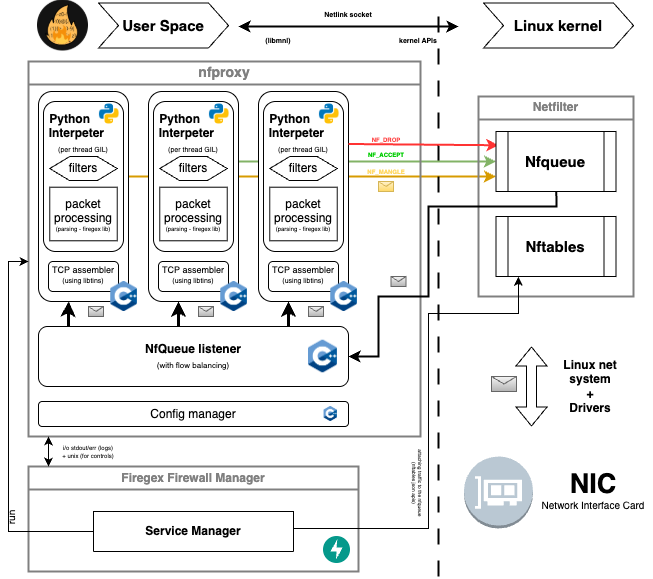
\includegraphics[width=0.9\textwidth]{images/chapter3/nfproxy.drawio.png}
    \caption{Architettura del modulo nfqueue}\label{fig:firegex_nfproxy_arch}
\end{figure}

\section{Elaborazione parallelizzata dei pacchetti}

Uno dei principali ostacoli progettuali ha riguardato la parallelizzazione dei processi di elaborazione, legata a tre fattori critici:  
il funzionamento intrinseco di \texttt{nfqueue}, alcune peculiarità del linguaggio Python e l'integrazione ibrida C++/Python.\\
Tre obiettivi hanno guidato l'implementazione della parallelizzazione:  

\begin{itemize}
    \setlength{\itemsep}{2pt}
    \setlength{\parskip}{2pt}
    \item \textbf{Isolamento dei dati tra processi}: Prevenire conflitti interprocesso per evitare corruzione dati, crash imprevisti e comportamenti anomali
    \item \textbf{Minimizzazione dei lock}: Limitare l'uso di meccanismi di blocco (pur necessari per risorse condivise) per prevenire deadlock e degradazione prestazionale
    \item \textbf{Ottimizzazione della memoria}: Eliminare copie ridondanti dei pacchetti e processi superflui, massimizzando throughput e riducendo latenza
\end{itemize}

La soluzione adottata segue il pattern produttore-consumatore. Un processo produttore unico, responsabile del binding alla \texttt{nfqueue},
riceve i pacchetti dal kernel e li distribuisce a multiple code FIFO.\@ I consumatori, associati ciascuno ad una coda dedicata, gestiscono in parallelo:
\begin{itemize}
    \setlength{\itemsep}{2pt}
    \setlength{\parskip}{2pt}
    \item Ordinamento dei pacchetti TCP  
    \item Applicazione dei filtri Python  
    \item Invio dei \texttt{verdicts}\footcite{\url{https://netfilter.org/projects/libnetfilter_queue/doxygen/html/group__nfq__verd.html}}{vedicts_nfqueue} al kernel
\end{itemize}

L'unica sezione critica risiede nell'accesso concorrente alle code, protetto da un sistema di lock basato su
\texttt{std::mutex}\footcite{\url{https://en.cppreference.com/w/cpp/thread/mutex}}{std_mutex} e \texttt{std::condition\_variable}\footcite{\url{https://en.cppreference.com/w/cpp/thread/condition_variable}}{condition_variable_std}.Questa scelta, preferita alle \texttt{unix pipe}\footcite{\url{https://man7.org/linux/man-pages/man2/pipe.2.html}}{unix_pipe} per motivi prestazionali, implementa un meccanismo di \texttt{backpressure} che blocca il produttore in caso di code sature, prevenendo consumo eccessivo di memoria.

L'implementazione si basa su quella pubblicata da \texttt{Arif Jaffer}\footcite{\url{https://www.bit-byter.com/blog/files/blocking-q-cpp.html}}{blocking_queue_cpp} per le code bloccanti.

\subsection{A Per-Interpreter GIL con python 3.12}

Una delle problematiche citate precedentemente sulla parallelizzazione riguardava una caratteristica del linguaggio Python: il \texttt{GIL}\footcite{Understanding the python gil}{beazley2010understanding} (Global Interpreter Lock). Questo meccanismo limita l'utilizzo dei thread consentendo l'esecuzione di un solo thread alla volta, necessario per prevenire conflitti nella gestione interna degli oggetti Python (come il reference counting) che non è implementata in modo thread-safe.

Si osserva inoltre come, nello specifico contesto, Python gestisca operazioni \emph{CPU-bound}, accentuando ulteriormente gli svantaggi del GIL.\@

\begin{figure}[H]
    \centering
    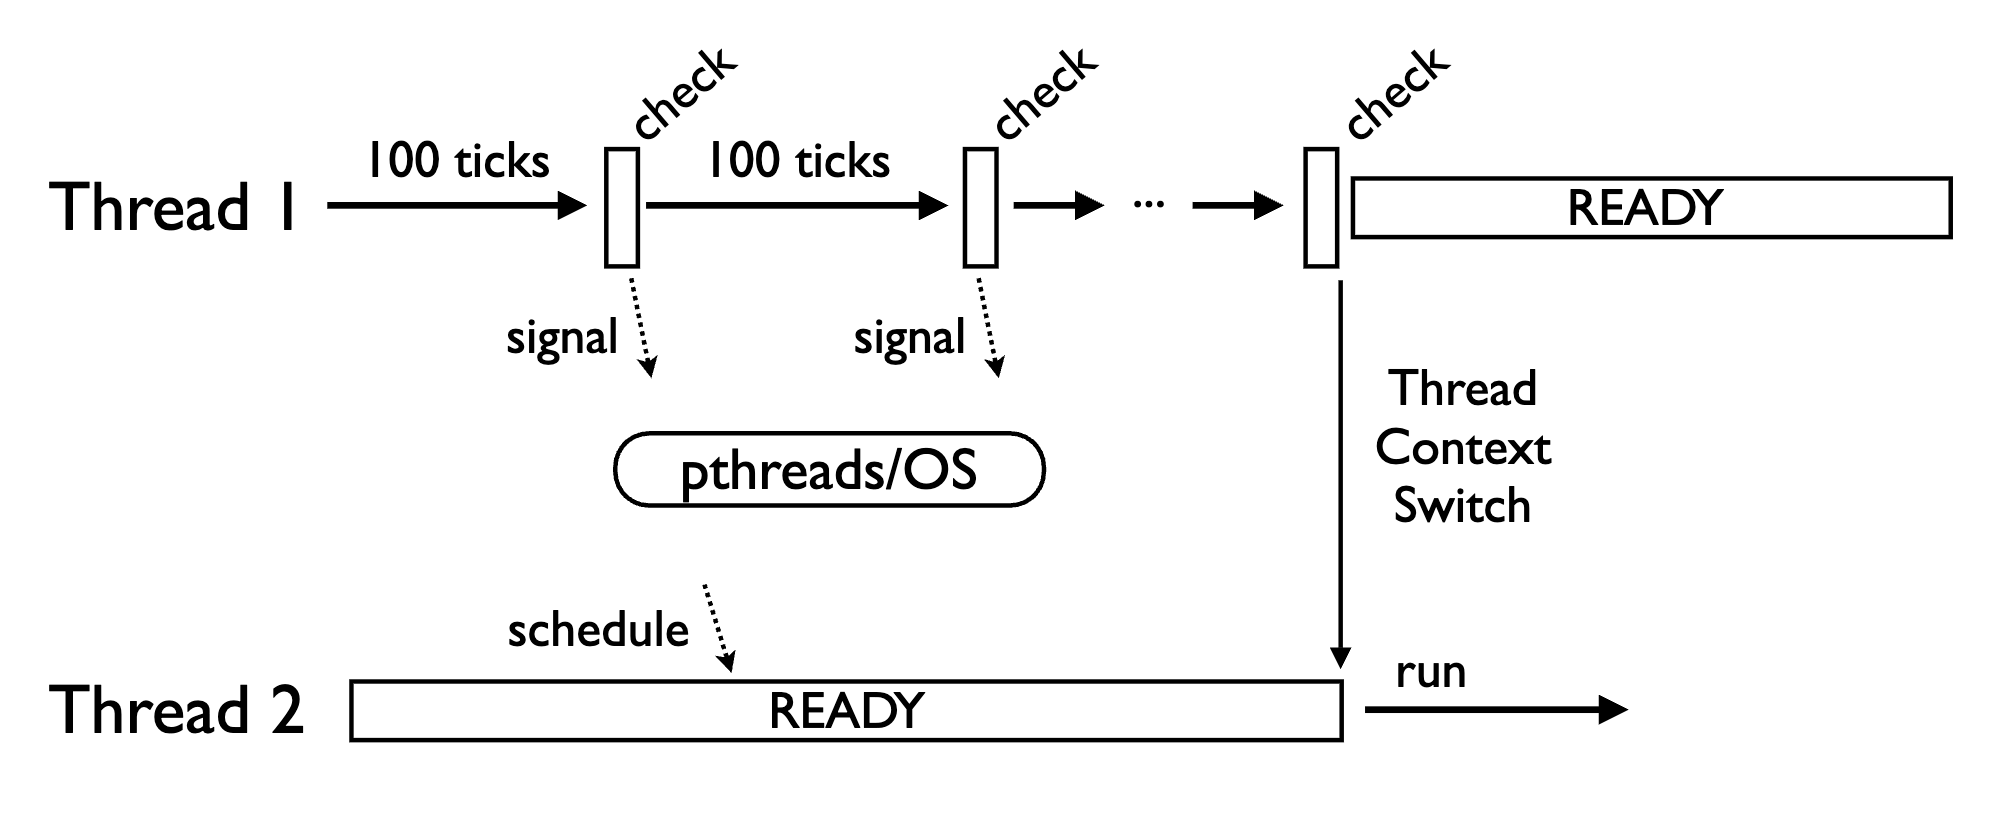
\includegraphics[width=0.98\textwidth]{images/chapter3/GIL.png}
    \caption{Python Global Interpreter Lock}\label{fig:py_gil_schema}
\end{figure}

Una soluzione alternativa potrebbe essere l'uso di processi multipli (con GIL separati per processo), approccio che tuttavia introdurrebbe overhead dovuti
alla comunicazione inter-processo e alla duplicazione della memoria.

La soluzione adottata sfrutta il \texttt{PEP 684}\footcite{\url{https://peps.python.org/pep-0684/}}{pep648} introdotto in Python 3.12, che permette l'esecuzione
di interpreti Python indipendenti nello stesso processo, ciascuno con il proprio GIL.\@ L'attivazione di questa funzionalità avviene esclusivamente tramite C-API, consentendo:
\begin{itemize}
    \setlength{\itemsep}{2pt}
    \setlength{\parskip}{2pt}
    \item Avvio diretto di interpreti via \texttt{libpython}
    \item Integrazione trasparente tra codice C++ e Python
    \item Parallelismo reale senza overhead di processi multipli
\end{itemize}

Il principale limite di questo approccio, cioè l'impossibilità di condividere oggetti tra interpreti, non costituisce un problema nel nostro caso poichè, grazie al meccanismo di
smistamento dei pacchetti descritto nel prossimo paragrafo, ciò non sarà necessario.\\
Per ogni nuova connessione TCP vengono eseguite le seguenti operazioni:\@
\begin{itemize}
    \setlength{\itemsep}{2pt}
    \setlength{\parskip}{2pt}
    \item Viene inizializzato un nuovo contesto globale Python indipendente
    \item Il bytecode del filtro viene deserializzato con \texttt{marshal}\footcite{\url{https://docs.python.org/3/library/marshal.html}}{marshal_python}
    \item Il codice di inizializzazione del filtro viene eseguito sul contesto globale
\end{itemize}

Qui viene riportato il codice di inizializzazione del consumatore con il relativo interprete Python indipendente.

\begin{listing}[H]
\begin{minted}[
    frame=single,
    framerule=0.8pt,
    fontsize=\footnotesize,
    breaklines
  ]{cpp}
// Configurazione interprete con GIL indipendente
PyInterpreterConfig py_thread_config = {
    .use_main_obmalloc = 0,
    .allow_fork = 0,
    .allow_exec = 0,
    .allow_threads = 0,
    .allow_daemon_threads = 0,
    .check_multi_interp_extensions = 1,
    .gil = PyInterpreterConfig_OWN_GIL,
};

void before_loop() {
    PyStatus pystatus;
    tstate = PyThreadState_New(PyInterpreterState_Main());
    PyEval_AcquireThread(tstate); // Acquisizione GIL
    pystatus = Py_NewInterpreterFromConfig(&tstate, &py_thread_config);
    handle_packet_code = unmarshal_code(...); // Deserializzazione bytecode
}
\end{minted}
\end{listing}

L'utilizzo delle funzionalità offerte dal \texttt{PEP 684}\footcite{\url{https://peps.python.org/pep-0684/}}{pep648}, soffre tuttavia di forti limitazioni sull'utilizzo di moduli non compatibili con la \texttt{multi-phase initialization}\footcite{\url{https://peps.python.org/pep-0489/}}{pep489} (includendo tutti quelli scritti in \texttt{Cython}\footcite{\url{https://cython.org/}}{cython}) e moduli con componenti non thread-safe. Nel corso dello sviluppo, queste limitazioni sono state oggetto di diverse problematiche, affrontate e approfondite in seguito.\\

Un'altra possibilità considerata è stata l'utilizzo dell'interprete in \texttt{free-threaded mode} di Python 3.13\footcite{\url{https://docs.python.org/3/whatsnew/3.13.html\#whatsnew313-free-threaded-cpython}}{py13_free_threaded}, attualmente sconsigliato per:
\begin{itemize}
    \setlength{\itemsep}{2pt}
    \setlength{\parskip}{2pt}
    \item Lo stato sperimentale della feature
    \item Calo prestazionale dovuto alla disattivazione temporanea di alcuni sistemi di ottimizzazione del linguaggio
    \item Incompatibilità con molti moduli CPython
\end{itemize}

\subsection{Bilanciamento del carico}

Per il bilanciamento del carico tra i processi consumatori, finalizzato all'isolamento e alla distribuzione equa dei pacchetti, è stato implementato un meccanismo di hashing basato su indirizzi IP e porte di origine/destinazione. Questo approccio garantisce una distribuzione uniforme dei pacchetti tra i consumatori, evitando sovraccarichi e assicurando un'elaborazione parallela efficiente, oltre che a instradare i pacchetti di una stessa connessione sempre verso lo stesso thread.\\

\begin{listing}[H]
\begin{minted}[
    frame=single,
    framerule=0.8pt,
    fontsize=\footnotesize,
    breaklines
  ]{cpp}
// Funzione di hashing per stream_id (valida per IPv4/IPv6)
uint32_t hash_stream_id(const stream_id &sid) {
    uint32_t addr_hash = 0;
    addr_hash ^= min_addr[0] ^ min_addr[1] ^ min_addr[2] ^ min_addr[3];
    addr_hash ^= max_addr[0] ^ max_addr[1] ^ max_addr[2] ^ max_addr[3];
    uint32_t ports = (static_cast<uint32_t>(sid.min_address_port) << 16) | sid.max_address_port;
    uint32_t hash = addr_hash ^ ports;
    hash *= 0x9e3779b9; // Aggiunta di entropia (moltiplicazione con numero primo)
    return hash;
}

// Funzione di bilanciamento semplificata
void __real_handler(PktRequest<Worker>* pkt) {
    const size_t idx = hash_stream_id(pkt->sid) % pkt->ctx->size();
    converted_pkt->ctx->queue.put(converted_pkt);
}
\end{minted}
\end{listing}

La tecnica riprende i meccanismi di bilanciamento usati kernel space da \texttt{nfqueue}, che tuttavia non considera le porte di origine/destinazione,
limitandosi ad un hashing basato solo sugli indirizzi IP.\@ Ciò è dovuto alla necessità di adattare l'algoritmo anche a protocolli diversi da TCP e UDP, come ICMP che non prevede porte.

\begin{listing}[H]
\begin{minted}[
    frame=single,
    framerule=0.8pt,
    fontsize=\footnotesize,
    breaklines
  ]{cpp}
// Codice estratto dal kernel Linux (versione 6.14-rc7)
static inline u32
nfqueue_hash(const struct sk_buff *skb, u16 queue, u16 queues_total, u8 family,
	     u32 initval)
{
	switch (family) {
	case NFPROTO_IPV4:
		queue += reciprocal_scale(hash_v4(ip_hdr(skb), initval),
					  queues_total);
		break;
	case NFPROTO_IPV6:
		queue += reciprocal_scale(hash_v6(ipv6_hdr(skb), initval),
					  queues_total);
		break;
	case NFPROTO_BRIDGE:
		queue += reciprocal_scale(hash_bridge(skb, initval),
					  queues_total);
		break;
	}
	return queue;
}
\end{minted}
\end{listing}

L'esclusione delle porte nell'hashing kernel\footnote{\url{https://web.git.kernel.org/pub/scm/linux/kernel/git/torvalds/linux.git/tree/include/net/netfilter/nf_queue.h?h=v6.14-rc7\#n105}}
nel sistema di balancing\footnote{\url{https://web.git.kernel.org/pub/scm/linux/kernel/git/torvalds/linux.git/tree/net/netfilter/xt_NFQUEUE.c?h=v6.14-rc7\#n86}} integrato in \texttt{nfqueue}
rappresenta un limite critico in scenari CTF con NAT, dove tutto il traffico anonimizzato verrebbe gestito da un singolo consumatore.
Questo è il motivo che ha spinto alla scelta di un approccio più sofisticato, che garantisce un effettivo bilanciamento del carico sui vari thread.

I benchmark su nfregex con carico simulato mostrano il beneficio che può portare questo sistema, come mostrato in Figura~\ref{fig:nfproxy_multithread_benchmark}.

\begin{listing}[H]
\begin{minted}[
    frame=single,
    framerule=0.8pt,
    fontsize=\footnotesize,
    breaklines
  ]{cpp}
// Simulazione carico computazionale usato nel benchmark
volatile int x = 0;
for (int i=0; i<50000; i++){
    x+=1;
}
\end{minted}
\end{listing}

\begin{figure}[H]
    \centering
    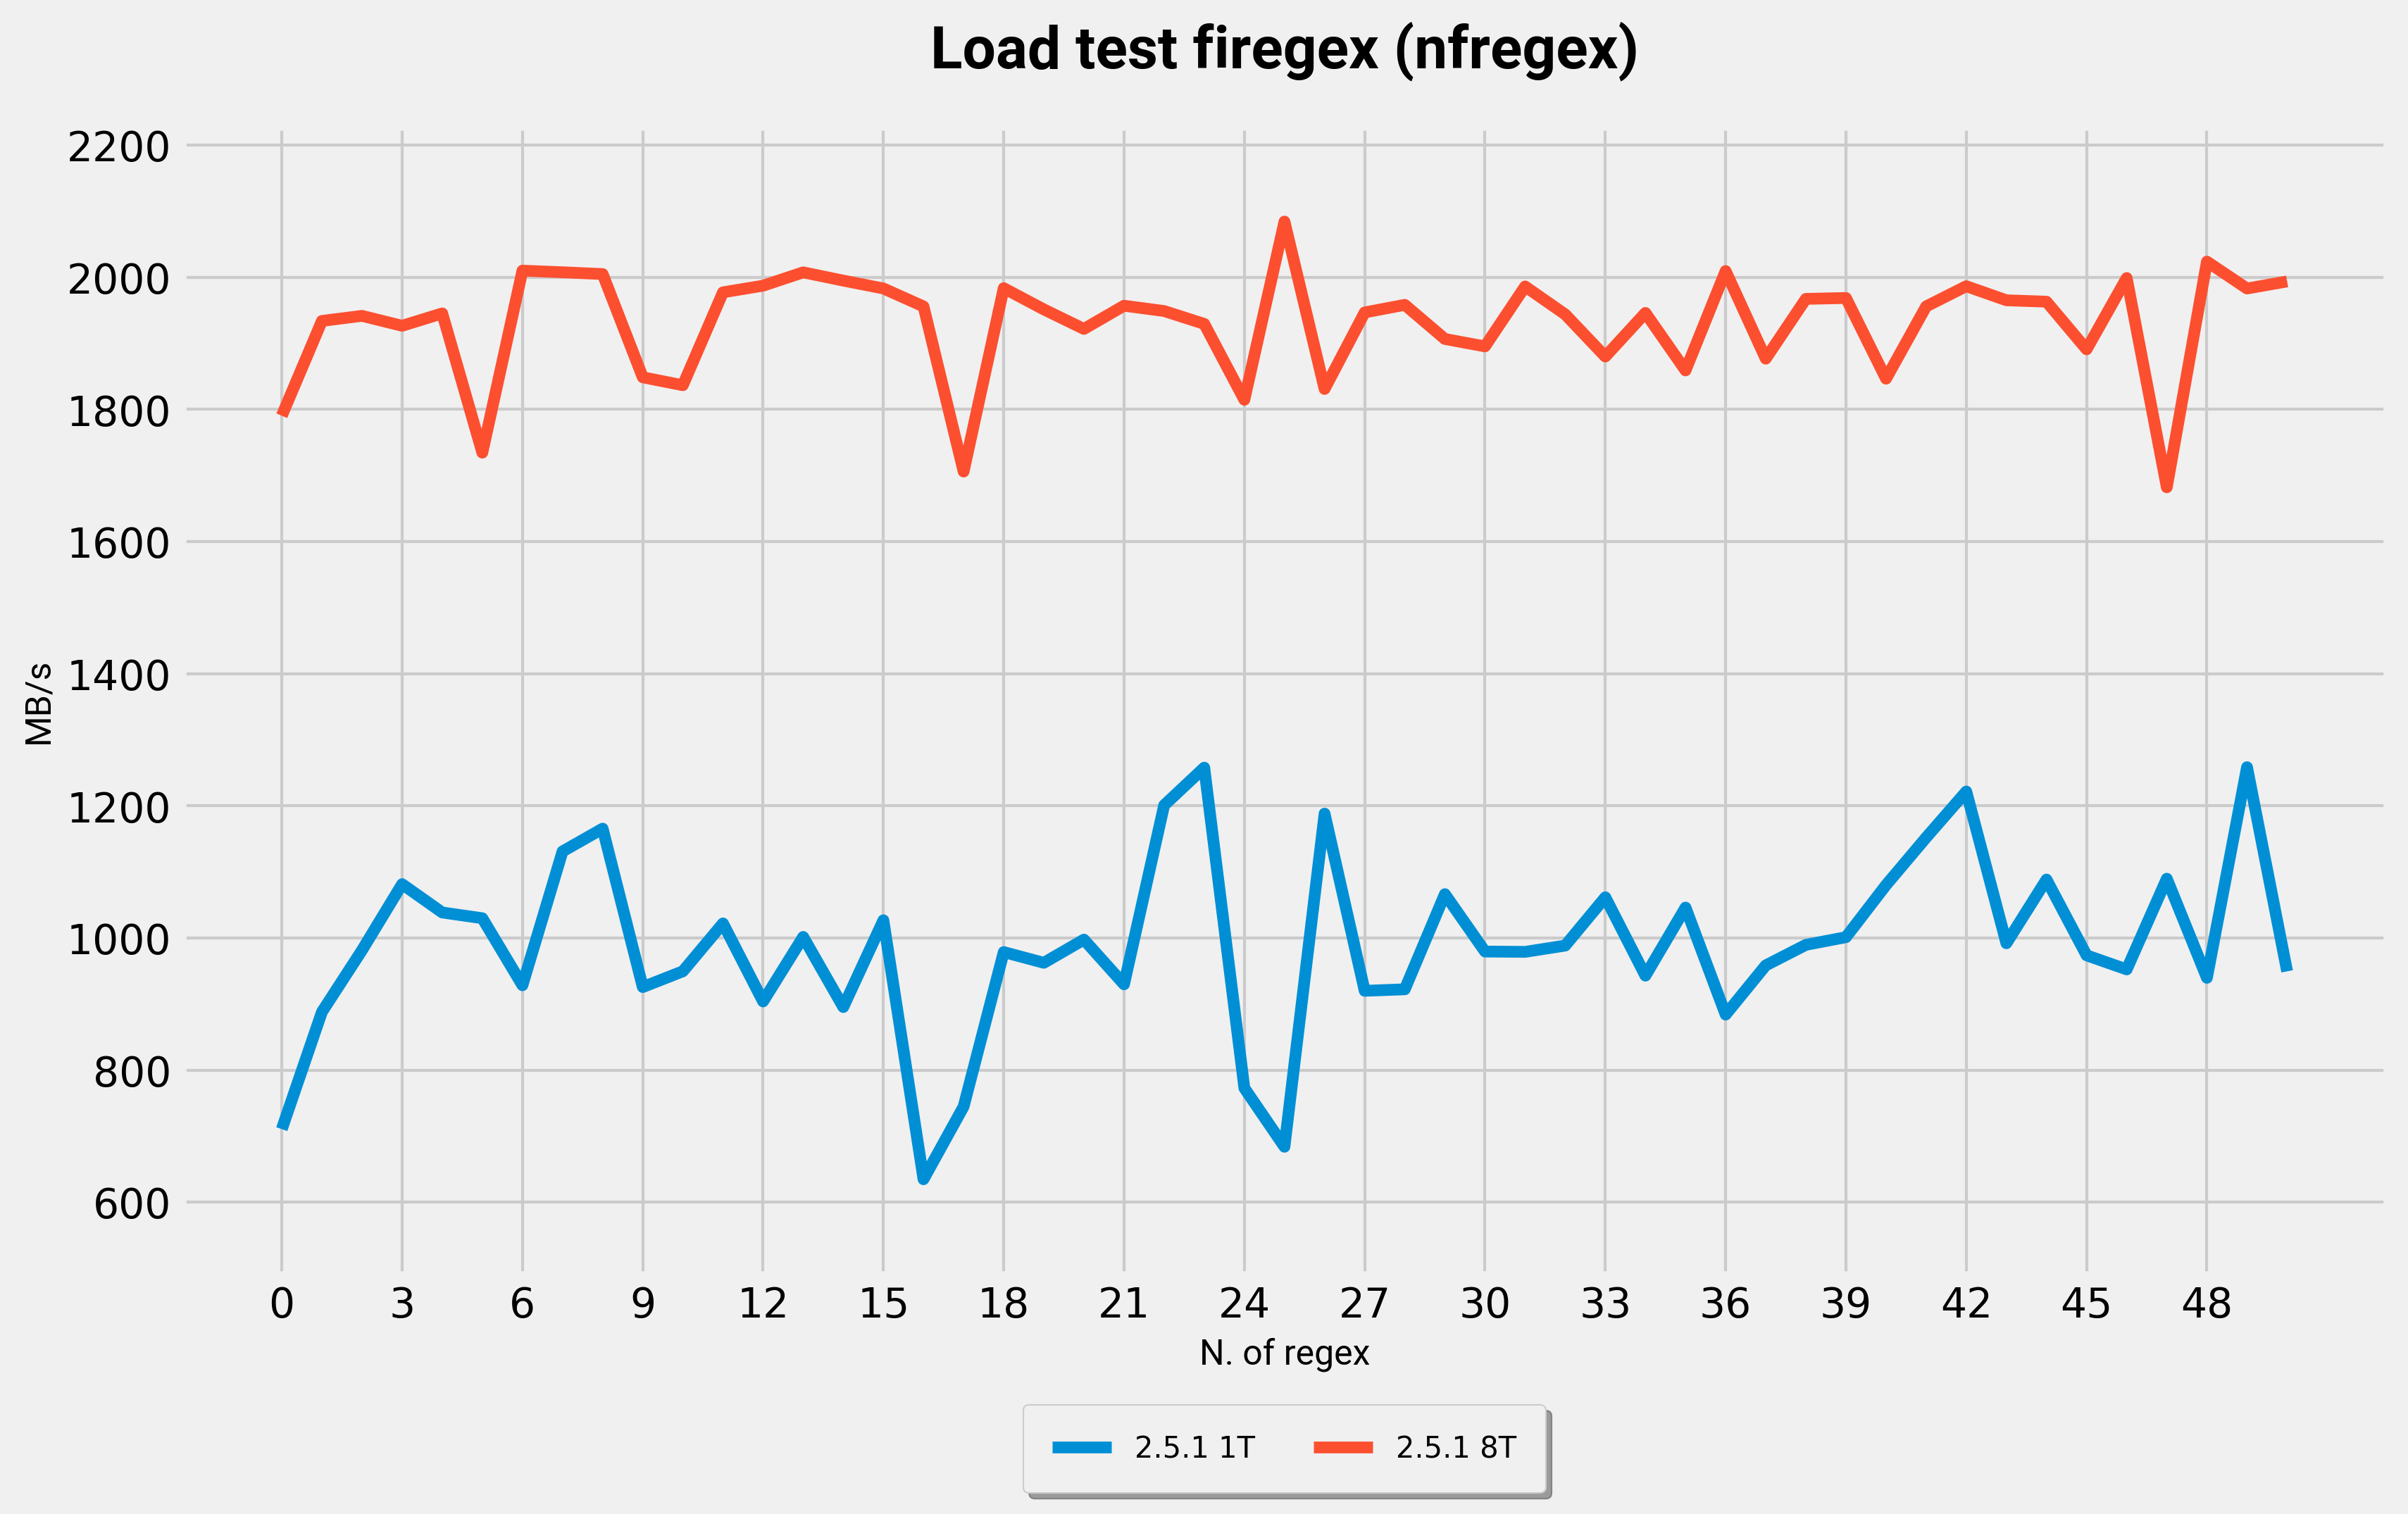
\includegraphics[width=0.98\textwidth]{images/chapter3/Benchmark-chart-with-load.png}
    \caption{Benchmark di NfProxy con load balancing personalizzato (1 vs 8 thread)}\label{fig:nfproxy_multithread_benchmark}
\end{figure}

I medesimi vantaggi prestazionali si possono riscontrare in nfproxy, che condivide la stessa base di codice per l'implementazione del bilanciamento del carico.

\section{Parsing dei pacchetti L3}

All'arrivo dei pacchetti nella \texttt{nfqueue}, viene eseguita un'analisi immediata del protocollo di livello 3 mediante ispezione dei primi
4 bit del campo \texttt{version}, valida sia per IPv4 che IPv6. Identificata la versione IP, il parsing multilivello viene delegato a
\texttt{libtins}\footcite{\url{https://libtins.github.io/}}{libtins}, che ricostruisce ricorsivamente gli header di rete e trasporto. 

La libreria genera automaticamente lo \texttt{stream\_id}, struttura dati univoca per identificare connessioni TCP/UDP attraverso
una coppia di tuple (IP:porta) sorgente/destinazione, che sono ordinate considerano la singola tupla come unica entità, e quindi non slegando mai
IP e porta tra loro. Questo approccio permette di identificare univocamente una connessione, indipendentemente dalla direzione del traffico (ingresso/uscita).

\begin{listing}[H]
\begin{minted}[
    frame=single,
    framerule=0.8pt,
    fontsize=\footnotesize,
    breaklines
  ]{cpp}
// Costruttore PktRequest: gestione pacchetti tra produttore/consumatore
PktRequest(const char* payload, size_t plen, T* ctx, mnl_socket* nl, 
           nfgenmsg *nfg, nfqnl_msg_packet_hdr *ph, bool is_input):
    ctx(ctx), nl(nl), res_id(nfg->res_id),
    packet_id(ph->packet_id), is_input(is_input),
    packet(string(payload, plen)),
    action(FilterAction::NOACTION),
    is_ipv6((payload[0] & 0xf0) == 0x60) // Verifica versione IP
{
    if (is_ipv6){
        ipv6 = new Tins::IPv6((uint8_t*)packet.c_str(), plen); // Parsing IPv6
        sid = stream_id::make_identifier(*ipv6); // Generazione stream_id
        _original_size = ipv6->size();
    }else{
        ipv4 = new Tins::IP((uint8_t*)packet.c_str(), plen); // Parsing IPv4
        sid = stream_id::make_identifier(*ipv4); 
        _original_size = ipv4->size();
    }
    l4_proto = fill_l4_info(); // Estrazione info layer 4
}
\end{minted}
\end{listing}

Inoltre lo \texttt{stream\_id} è indipendente dal protocollo internet utilizzato, permettendo di identificare connessioni miste IPv4/IPv6: questo permette di utilizzare la stessa queue per interfaccie di rete differenti, carattertistica potenzialmente utile per implementare nuove feature sulla selezione del traffico da inoltrare alla queue.\\

Ogni produttore utilizza questo dato come chiave per individurare i dati relativi ad una specifica connessione, salvandoli in una \texttt{std::map}\footcite{\url{https://en.cppreference.com/w/cpp/container/map}}{std_map} diversa per ogni singolo produttore, così implementabile per merito del meccanismo di smistamento dei pacchetti descritto precedentemente.\\

Il produttore, ricevuto il pacchetto, lo ingloba in un oggetto \texttt{PktRequest}, che contiene tutte le informazioni necessarie per l'elaborazione del pacchetto, e lo inserisce nella coda condivisa del produttore di riferimento.\\
Sarà il produttore che una volta elaborato il pacchetto ed inviato il verdetto al kernel, deallocherà questa struttura passando all'elaborazione del prossimo pacchetto. Nessuna copia in memoria è pertanto necessaria in questo passaggio.

\section{Gestione dei pacchetti TCP}

Come citato precedentemete, prima di inizializzare la queue, vengono inseriti tramite nftables le regole per intercettare il traffico in un certo punto della catena di netfilter, per essere mandato alla queue che determinerà un verdetto sul pacchetto.\\

\begin{figure}[H]
    \centering
    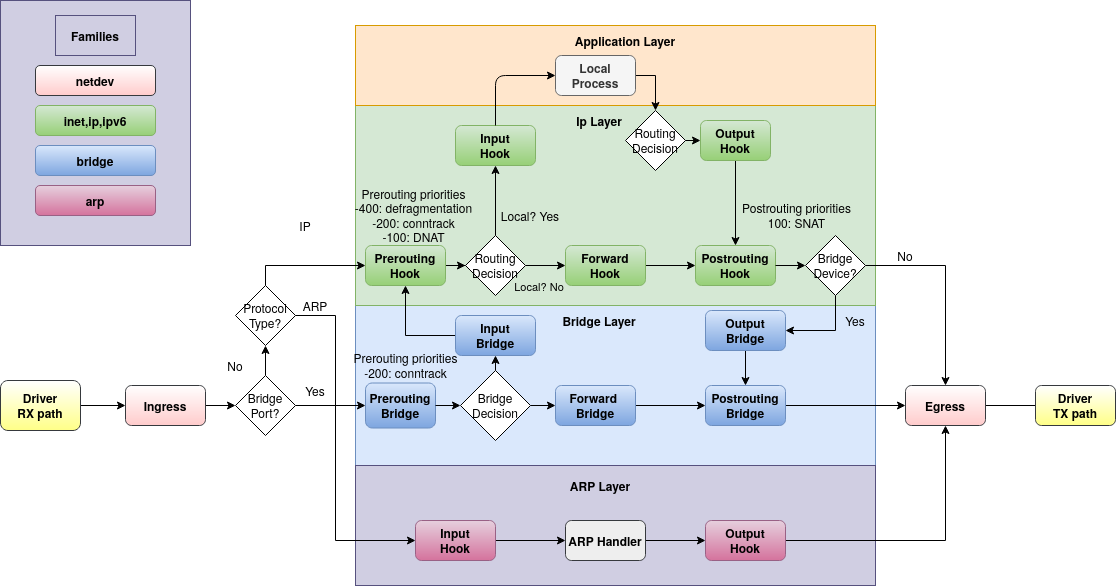
\includegraphics[width=0.98\textwidth]{images/chapter3/nf-hooks.png}
    \caption{NfTables Hooks}\label{fig:nftables_hooks}
\end{figure}

Il traffico in particolare viene intercettato sia in \texttt{pre-routing}, che in \texttt{post-ruoting} ad un hook prima dell'azione del modulo conntrack, ma dopo dell'azione di defrag, in particolare a prio -310 che rientra in questo range come riportato sulla \texttt{wiki ufficiale di nftables}\footcite{\url{https://wiki.nftables.org/wiki-nftables/index.php/Netfilter_hooks}}{netfilter_hooks}. Questo permette di ottenere dei pacchetti che hanno già subito il processo di deframmentazione a livello 3, di cui pertanto non ci dovremo preoccupare, che non hanno subito il processo di routing (che quindi volendo potremmo manipolare) e che non sono stati ancora analizzati dal modulo conntrack.\\
Tuttavia, qui i pacchetti non hanno subito il processo di ordinamento dei payload che avviene a livello 4, sul quale come è possibile osservare dalla Figura~\ref{fig:nftables_hooks}, non è possibile intercettare del traffico, poiché i pacchetti arriveranno direttamente alle fasi di gestioni dei dati per la loro consegna alla socket a livello applicatvo.\\
Pertanto è dato a noi il compito di analizzare il traffico e di ordinare i pacchetti TCP per un'utilizzo dei dati coerente a quelli che saranno letti dall'applicazione.\\
\texttt{Libtins} semplifica significativamente questa gestione attraverso meccanismi automatizzati gestiti dal suo \texttt{TCP follower}\footnote{Esempio TCP Follower: \url{https://libtins.github.io/examples/http-requests/}} per:  
\begin{itemize}
    \setlength{\itemsep}{2pt}
    \item Chiusura dei flussi TCP basata su:
    \begin{itemize}
        \setlength{\itemsep}{1pt}
        \item Analisi del traffico (flag FIN/RST)
        \item Timeout configurabili
        \item Rilevamento di inattività prolungata
    \end{itemize}
    \item Ricostruzione dello stream da segmenti non ordinati
    \item Gestione automatica dei buffer con prevenzione su memory leak
\end{itemize}

Il follower inoltre permette facilmente l'integrazione di dati gestiti esternamente, tramite il suo sistema di callback, che ne chiamerà le funzionalità compatibilmente con quanto fatto con i buffer internamente.\\
Le callback permettono di gestire le seguenti operazioni:
\begin{itemize}
    \setlength{\itemsep}{2pt}
    \item Inizializzazione contesti
    \item Pulizia risorse
    \item Propagazione di eventi critici (per chiusure anomale dei flussi)
\end{itemize}

Ogni processo consumatore ha un suo follower dedicato che analizzerà i flussi relativi alla porzione traffico a lui dedicata.

\section{Modifica dei pacchetti}

Il modulo \texttt{nfqueue} consente effettivamente la modifica dei pacchetti, offrendo potenzialmente la possibilità di alterare header
IP/TCP e payload a livello di trasporto. Tuttavia, questa funzionalità, seppur teoricamente disponibile, è stata implementata solo parzialmente e non risulta pienamente affidabile.\\
Le limitazioni derivano da problematiche intrinseche legate all’interazione con i meccanismi di livello di trasporto. Ad esempio, modifiche al payload TCP durante connessioni attive potrebbero invalidare checksum o causare inconsistenze nei sequence number. La complessità per garantire coerenza in tutti i possibili scenari (come in caso di ritrasmissioni) rende l’implementazione robusta di questa feature particolarmente onerosa. Inoltre, se gestita male, la modifica del payload potrebbe essere soggetta a vulnerabilità di sicurezza. Valutando il rapporto rischio-beneficio, si è optato per comunque rendere disponibile la funzionalità, seppur parzialmente implementata, ma fortemente disincentivata e volutamente resa meno facilmente accessibile.\\
L’effettiva necessità operativa risulta infatti marginale nella maggior parte degli scenari CTF, mentre i potenziali effetti collaterali verrebbero a compromettere uno degli obiettivi principali: la stabilità del servizio.\\
Di seguito si riporta una descrizione accurata delle problematiche riscontrate e delle soluzioni proposte, o applicate con relativi limiti e valutazioni rischio/beneficio.\\
\texttt{NOTA}: Le problematiche sul calcolo dei campi di integrità dei dati non sono trattate, ma considerate già risolte tramite l'utilizzo di libtins, che si occupa durante la serializzazione del pacchetto di ricalcolare questi campi nei vari layer interessati, pertanto non considerata una problematica rilevante.\\
L'unica operazione aggiuntiva affrontata su questo, è stata la necessità di reinserire il payload del pacchetto nella catena di PDU di libtins, poiché (seppur non documentato), il follower del flusso TCP internamente separa di fatto il payload dal pacchetto\footnote{Separazione del payload nel follower: \url{https://github.com/mfontanini/libtins/blob/b7e61f4c76ac64053c9c4c9f8eadaabbe3a9381a/src/tcp_ip/data_tracker.cpp\#L68}}, rendendone necessario il reinserimento per la corretta serializzazione e calcolo di questi campi.\\

\subsection{Cambio di dimensione del payload}

Come emerge dalle specifiche stesse del protocollo di trasporto TCP\footcite{RFC9293, Transmission Control Protocol (TCP)}{rfc9293}, questo tiene traccia dello stato della corretta recezione dei pacchetti tramite un meccanismo di \texttt{piggybacking} che fa utilizzo dei campi numerici ack e seq.
Nella trasmissione, il sequence number indica il byte da cui inizia il payload del pacchetto relativamente alla sua posizione nello stream, mentre il campo ack della risposta di conferma proveniente dal ricevente, indica fino a che punto il flusso di dati è stato ricevuto correttamente.\\
Questo meccanismo è fondamentale per il corretto funzionamento del protocollo e per la corretta ricostruzione del flusso originale: di conseguenza la modifica alla dimensione del payload causa inevitabilmente l'incoerenza di questi valori che porteranno a comportamenti inaspettati, non conformi al normale funzionamento del protocollo.\\

Per risolvere la problematica descritta, è stato implementato un sistema di traduzione bidirezionale dei campi \texttt{SEQ} (sequence number) e \texttt{ACK} (acknowledgment number).
Questo meccanismo garantisce la coerenza logica della comunicazione riconvertendo i valori modificati in modo da preservare la corrispondenza tra la dimensione originale dei pacchetti e le aspettative del client (ma anche del server).
Il kernel e il TCP Follower di \texttt{libtins} ricevono così numerazioni coerenti con le alterazioni applicate, mantenendo la sincronizzazione degli stati di connessione.
Il sistema opera in modo simmetrico per entrambe le direzioni del traffico: le modifiche applicate ai pacchetti in uscita vengono compensate da una riconversione inversa per quelli in entrata.
L'attivazione avviene automaticamente alla prima modifica di un pacchetto nella sessione TCP e rimane attiva per tutta la durata della connessione, garantendo la persistenza del contesto di traduzione.\\
La conversione degli ack e seq pertanto avviene tramite il calcolo incrementale dell'offset che intercorre tra la dimensione del flusso originale e la dimensione del flusso modificato,
calcolata incrementalmente come si può osservare nel seguente codice:

\begin{listing}[H]
    \begin{minted}[
        frame=single,
        framerule=0.8pt,
        fontsize=\footnotesize,
        breaklines
      ]{cpp}
size_t payload_offset = data_size() != _data_original_size;
// If we are in a TCP connection, the ack and seq status context was enabled, and the payload size 
if (tcp && ack_seq_offset && payload_offset != 0){
    // So we incrementally update the total offset based on who sent this data.
    if (is_input){
        ack_seq_offset->in += payload_offset;
    }else{
        ack_seq_offset->out += payload_offset;
    }
}
\end{minted}
\end{listing}

A seguito della modifica, nei prossimi pacchetti vengono compatibilmente ricalcolati gli ack e seq, su tutto il traffico come si può vedere nel seguente codice:

\begin{listing}[H]
    \begin{minted}[
        frame=single,
        framerule=0.8pt,
        fontsize=\footnotesize,
        breaklines
      ]{cpp}
void fix_tcp_ack(){
    // Checks if the conversion is needed
    need_tcp_fixing = need_tcp_fix();
    if(!need_tcp_fixing){
        return;
    }
    // conversion of the ack and seq
    if (is_input){
        tcp->seq(tcp->seq() + ack_seq_offset->in);
        tcp->ack_seq(tcp->ack_seq() - ack_seq_offset->out);
    }else{
        tcp->ack_seq(tcp->ack_seq() - ack_seq_offset->in);
        tcp->seq(tcp->seq() + ack_seq_offset->out);
    }
}
\end{minted}
\end{listing}


Un'analisi preliminare e test di base suggerirebbero l'adeguatezza di questa soluzione. Tuttavia occorre sottolineare come il meccanismo presenti limitazioni intrinseche in specifiche casistiche operative. L'approccio risulta efficace esclusivamente in condizioni ideali di trasmissione, dove non si verificano fenomeni di ritrasmissione di pacchetti persi né ricezione di segmenti non ordinati.\\

La criticità principale risiede nell'algoritmo di conversione, che non considera adeguatamente le ritrasmissioni di segmenti antecedenti al pacchetto modificato. In tali scenari, il calcolo dell'\texttt{ACK} relativo al segmento ritrasmesso richiederebbe una ricalibrazione temporale analoga a quella applicata ai pacchetti successivi, operazione che l'implementazione corrente non esegue. Questo deficit nasce dall'assenza di un modello contestuale capace di identificare la porzione di flusso effettivamente coinvolta nella ritrasmissione, portando a discrepanze cumulative negli stati di connessione che compromettono progressivamente la sincronizzazione degli endpoint.

\begin{figure}[H]
    \centering
    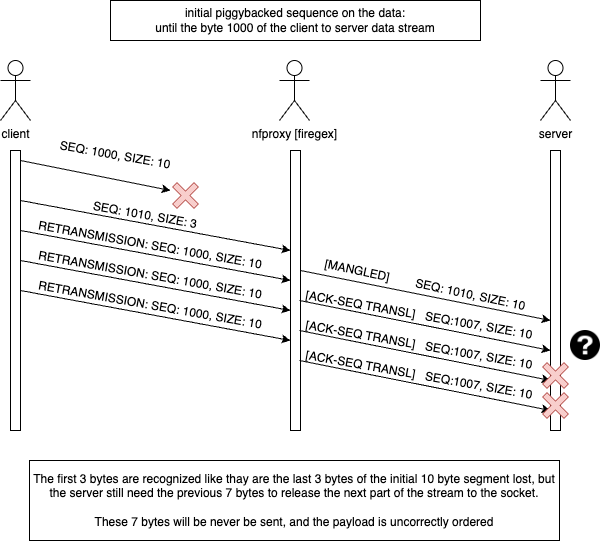
\includegraphics[width=0.90\textwidth]{images/chapter3/TCP_ack_seq_transl_failure.drawio.png}
    \caption{Esempio di una possibile problematica nella traduzione di ack e seq implementata}\label{fig:tcp_ack_seq_transl_failure}
\end{figure}

L'analisi della Figura~\ref{fig:tcp_ack_seq_transl_failure} evidenzia come le casistiche descritte possano compromettere integralmente il sistema di traduzione implementato. Tali scenari, particolarmente probabili in condizioni di congestione di rete, rappresentano potenziali vettori d'attacco mirati a destabilizzare il servizio.

Alla luce di queste considerazioni, si conclude che la soluzione proposta non possiede la robustezza necessaria per un'implementazione definitiva. La funzionalità di modifica pacchetti viene pertanto mantenuta come opzione sperimentale, accompagnata da avvertenze esplicite sul suo comportamento instabile.

Una soluzione teoricamente più solida richiederebbe la memorizzazione di informazioni aggiuntive riguardo i vari punti del flusso dove il traffico è stato modificato, insieme agli offset applicati in quegli specifici intervalli, per tutta la finestra di trasmissione ancora non riscontrata dal ricevente. Inoltre, sarebbe necessaria una logica di traduzione più complessa per gli \texttt{ACK}/\texttt{SEQ}, che vada ad esguire un calcolo corerente di questi valori, basato sul posizionamento che il segmento ha in trasmissione o riscontro nel flusso complessivo, sfruttando le nuove informazioni memorizzate.

Considerando il rapporto costo-beneficio e il limitato valore operativo della funzionalità, si è optato per mantenere lo stato corrente dello sviluppo, consapevoli delle possibili criticità che può portare, non essendo una soluzione definitiva.

\subsection{Modifica di segmenti non ordinati}

Un'ulteriore criticità emerge nella gestione dei pacchetti con payload \emph{out-of-order} da modificare. Nell'implementazione corrente, i pacchetti non ordinati vengono analizzati dal TCP Follower di \texttt{libtins} per la ricostruzione dello stream ed accettati immediatamente dopo questa elaborazione, privando tuttavia il sistema della possibilità di modificarli successivamente. Questo meccanismo, sebbene un payload malevolo venga accettato, riesce comunque a bloccarlo a livello applicativo, prima che il flusso possa essere completamente riordinato, intervenendo sul primo pacchetto disordinato, che causerebbe a quel punto la chiusura forzata della connessione.

Una soluzione alternativa prevedrebbe il buffering dei pacchetti \emph{out-of-order} in attesa dei segmenti mancanti, applicando modifiche retroattive sui pacchetti trattenuti. Tuttavia, questo approccio introdurrebbe: una complessità significativa nel meccanismo di ricostruzione distribuita del flusso e il rischio di saturare la \texttt{nfqueue} kernel-side, con conseguente perdita di pacchetti e possibile esposizione ad attacchi \texttt{DoS} mirati a sfruttare le debolezze di questo sistema, potenzialmente portandolo ad un blocco del traffico.

Sulla base di queste considerazioni, si conclude che il riscontro immediato dei pacchetti è un approccio che deve essere applicato al fine di scongiurare possibili criticità riguardanti il riempimento della coda kernel, soggetta a questa tipologia di attacchi. La scelta progettuale attuale, seppur limitante, garantisce un'operatività ed un throughput stabile e prevedibile, mantiene il sistema immune a possibili vulnerabilità ma non offre la possibilità di eseguire modifiche su pacchetti non ordinati.\\

Sarebbe possibile progettare un sistema che eviti i problemi di saturazione della coda kernel, implementando ad esempio un meccanismo basato su dei timeout che evitino la saturazione della coda eliminando i pacchetti potenzialmente fraudolenti. Tuttavia simili implementazioni richiederebbero un'attenta analisi ed uno studio molto più approfondito rispetto a quanto fatto finora, considerando anche un vasto spettro di casistiche insidiose che non si ritiene necessario affrontare in questa tesi e ai fini dello sviluppo di questo modulo.\\

\section{Parsing dei pacchetti HTTP}

Dall'analisi delle soluzioni esistenti per il parsing di pacchetti HTTP è emersa l'assenza di strumenti compatibili con i requisiti specifici del progetto, in particolare per quanto riguarda l'integrazione con le funzionalità introdotte dal \texttt{PEP 684}\footcite{\url{https://peps.python.org/pep-0684/}}{pep648}. La necessità di supportare l'inizializzazione multi-fase (multi-phase initialization\footcite{\url{https://peps.python.org/pep-0489/}}{pep489}) e garantire thread safety ha reso indispensabile un approccio personalizzato.

La soluzione adottata si basa su un fork modificato dell'implementazione di \texttt{Derrick Lyndon Pallas}\footcite{Python wrapper per llhttp: \url{https://github.com/pallas/pyllhttp}}{original_pyllhttp_impl}, che utilizza il parser \texttt{llhttp}\footcite{\url{https://github.com/nodejs/llhttp}}{llhttp} sviluppato per \texttt{Node.js}. Questo fork, pubblicamente disponibile su GitHub\footcite{\url{https://github.com/domysh/pyllhttp}}{pyllhttp_fork} e distribuito tramite PyPI\footnote{\texttt{https://pypi.org/project/pyllhttp/}} va a risolvere le limitazioni tecniche derivanti dalla sua versione originale e preserva le capacità core di llhttp, tra cui il parsing zero-copy dei chunk, e la validazione rigorosa dello standard \texttt{HTTP/1.1}\footcite{RFC2616, Hypertext Transfer Protocol -- HTTP/1.1}{rfc2616}.

\subsection{Supporto agli algoritmi di compressione HTTP}

Nel traffico HTTP sono spesso in uso algoritmi di compressione per ridurre la dimensione del body. Dato il loro ampio utilizzo, al fine di semplificare l'implementazione di filtri ne richiederebbero l'analisi del contenuto, si è deciso si supportare la decompressione automatica degli algoritmi supportati dal browser \texttt{chrome}:

\begin{itemize}
    \setlength{\itemsep}{2pt}
    \setlength{\parskip}{2pt}
    \item \textbf{gzip}\footcite{RFC1952, GZIP file format specification version 4.3}{rfc1952}: Nativamente supportato in python.
    \item \textbf{brotli}\footcite{RFC7932, Brotli Compressed Data Format}{rfc7932}: supportato tramite un'implementazione eseguita da \texttt{google}\footcite{\url{https://github.com/google/brotli}}{brotli_gh}, che tuttavia non supporta il \texttt{PEP 684}, per cui anche in questo caso è stato sviluppato un fork compatibile disponibile su github\footcite{\url{https://github.com/domysh/brotli}}{brotli_fork}.
    \item \textbf{zstd}\footcite{RFC8478, Zstandard Compression and the application/zstd Media Type}{rfc8478}: supportato tramite un wrapper python sviluppato da \texttt{Sergey Dryabzhinsky}\footcite{\url{https://github.com/sergey-dryabzhinsky/python-zstd}}{zstd_ortiginal_python_wrapper}, che tuttavia, essendo anch'esso non compatibile con il \texttt{PEP 684}, è stato personalizzato in un ulteriore fork\footcite{\url{https://github.com/domysh/python-zstd}}{zstd_fork}.
    \item \textbf{deflate}\footcite{RFC1951, DEFLATE Compressed Data Format Specification version 1.3}{rfc1951}: Implementabile tramite il modulo \texttt{zlib}.
\end{itemize}

L'implementazione è stata scritta seguendo le specifiche definite nell'\texttt{RFC 2616} il quale definisce la possibilità di compressioni multiple, correttamente supportate nell'implementazione finale.
    
\subsection{Supporto alle websocket}

Nell'implementazione per HTTP/1.1 è stato incluso anche il supporto alle \texttt{websocket}\footcite{RFC6455, The WebSocket Protocol}{rfc6455}, tramite l'utilizzo della principale libreria python utilizzata per le decodifica dei \texttt{Frame}, ovvero \texttt{websockets}\footcite{\url{https://websockets.readthedocs.io/en/stable/}}{python_websockets}. Da qui sono state prese le funzionalità di decodifica dei frame, e le funzionalità per il supporto all'estensione \texttt{permessage-deflate}\footcite{RFC7692, Compression Extensions for WebSocket}{rfc7692}, per permetterne la decompressione, utilizzando internamente \texttt{zlib}, già resa compatibile per \texttt{PEP 684} grazie al fork precedentemente citato. La complessità nell'implementazione delle websocket si è concentrata sulla necessità di assemblare il flusso di dati correttamente, dato il mancato supporto nativo al parsing in streaming, come invece supportato su \texttt{llhttp}. Nella fase di upgrading della connessione HTTP, vengono riconosciuti i plugin abilitati, e viene automaticamente introdotta la gestione dei websocket che si occupa di decodificare i prossimi dati sulla connessione TCP.\\
In caso di fallimento nel parsing dei frame, i dati vengono resi disponibili per il filtraggio, semplicemente come byte grezzi, stesso meccanismo usato in caso di upgrade ad HTTP/2 (non supportato attualmente).

\section{Sintassi e gestione dei filtri python}



I filtri Python per \texttt{nfproxy} vengono definiti in file singoli (uno per servizio) contenenti funzioni annotate con il decoratore \texttt{@pyfilter}. Queste funzioni, denominate collettivamente \texttt{pyfilters}, accettano parametri tipizzati che rappresentano i dati estratti dal traffico di rete e restituiscono istruzioni di azione (\texttt{ACCEPT}, \texttt{REJECT}, \texttt{DROP}, chiamati \texttt{statment}) determinando il comportamento finale sul pacchetto.  

L'esempio seguente illustra un filtro che blocca le richieste HTTP contenenti la stringa `\texttt{curl}' nell'header \texttt{User-Agent} e impedisce gli upgrade a WebSocket:

\begin{listing}[H]
    \begin{minted}[
        frame=single,
        framerule=0.8pt,
        fontsize=\footnotesize,
        breaklines
      ]{python}
from firegex.nfproxy.models import HttpRequest
from firegex.nfproxy import pyfilter, REJECT

@pyfilter
def curl_filter(r: HttpRequest):
    if r.upgrading_to_ws:
        return REJECT  # Blocca upgrade a WebSocket
    if "curl" in r.user_agent:
        print(f"Tentativo accesso con curl: {r.user_agent}")
        return REJECT  # Blocca client curl
\end{minted}
\end{listing}

Il sistema si appoggia alla libreria \texttt{firegex}\footcite{\url{https://pypi.org/project/firegex/}}{firegex_pypi}, che fornisce sia i decoratori per la definizione dei filtri, sia i modelli dati per l'annotazione dei parametri. Durante la fase di compilazione, \texttt{nfproxy} analizza staticamente le signature delle funzioni, sullo stesso principio di validazione tipica di \texttt{pydantic}\footcite{\url{https://docs.pydantic.dev/latest/}}{pydantic}, per determinare automaticamente quali layer di protocollo analizzare (es. HTTP, TCP), eventalmente quali campi estrarre dal payload, attivando internamente una serie di meccanismi per riuscire a soddisfare le richieste dei filtri.\\
Se un filtro richiede dati non coerenti tra loro, potrebbe essere elaborato ma mai di fatto eseguito.
L'esecuzione avviene tramite dispatch dinamico: a ogni pacchetto corrispondente ai criteri dichiarati nella signature vengono passati gli oggetti istanziati se disponibili, e ne viene successivamente dato un riscontro sull'azione da eseguire tramite il valore di ritorno. L'assenza di un'istruzione \texttt{return} o il ritorno esplicito di \texttt{None} equivalgono a un'azione \texttt{ACCEPT} implicita.\\
I filtri continuano ad essere eseguiti fino a che tutti quelli attivi non vengono elaborati, o fino a che uno statment diverso da \texttt{ACCEPT} viene restituito.
Le funzionalità per la modifica del traffico sono accessibili tramite lo statment \texttt{UNSTABLE\_MANGLE}, che si occuperà di elaborare le modifiche eseguite al pacchetto, tramite il model \texttt{RawPacket}. Eventuali modifiche tuttavia non andranno ad influenzare gli altri datahandler che non le riveleranno.

Ulteriori dettagli sull'utilizzo dei models (spesso chiamati anche datahandler) sono disponibili nella documentazione integrata nell'interfaccia di \texttt{firegex}.

\subsection{Gestione dei buffer di memoria}

La gestione di flussi di traffico con payload di grandi dimensioni richiede un'attenzione particolare al consumo di memoria, specialmente in contesti ad alto throughput. \texttt{nfproxy} implementa un sistema di bufferring che consente una dimensione massima predefinita di 1MB per ciascun tipo di \texttt{datahandler}, tentando di mantere il corretto funzionamento dei parser anche in condizioni di sovraccarico. Infatti quando la soglia viene superata, il buffer viene automaticamente svuotato sebbene ciò possa comportare perdita di informazioni utili.

Il comportamento predefinito è configurabile attraverso variabili globali che permettono di adattare il bilanciamento tra consumo di risorse e completezza analitica. È possibile ridurre la dimensione massima dei buffer per ambienti memory-constrained o aumentarla per scenari che richiedono la ricostruzione completa di flussi complessi. In aggiunta, l'azione da intraprendere al superamento della capacità del buffer può essere personalizzata tra quattro opzioni: svuotamento controllato (\texttt{FLUSH}), accettazione passiva del traffico successivo (\texttt{ACCEPT}), rifiuto selettivo della connessione (\texttt{REJECT}), o drop dei pacchetti successivi (\texttt{DROP}).

Il seguente estratto dalla documentazione ufficiale illustra la configurazione avanzata tramite variabili globali, dimostrando come ottimizzare il sistema per flussi tipici di 4KB:\@

\begin{listing}[H]
    \begin{minted}[
        frame=single,
        framerule=0.8pt,
        fontsize=\footnotesize,
        breaklines
      ]{python}
from firegex.nfproxy import FullStreamAction

FGEX_STREAM_MAX_SIZE = 4096  # Limite dimensionale per tipo di datahandler
FGEX_FULL_STREAM_ACTION = FullStreamAction.REJECT  # Politica di overflow

# Configurazione ottimizzata per flussi medio-piccoli
# Connessioni che superano 4KB vengono chiuse preventivamente
\end{minted}
\end{listing}

\section{Proxy di simulazione}

Per validare il corretto funzionamento dei filtri prima del deployment sul firewall, \texttt{firegex} integra un ambiente di simulazione basato su proxy TCP.\@ Questo strumento, accessibile tramite il comando \texttt{fgex nfproxy}, consente di testare le regole in condizioni controllate riproducendo fedelmente l'architettura operativa del modulo reale.\\
Un tipico workflow di testing prevede l'esecuzione di un comando simile al seguente:
\begin{listing}[H]
    \begin{minted}[
        frame=single,
        framerule=0.8pt,
        fontsize=\footnotesize,
        breaklines
      ]{bash}
fgex nfproxy test_http.py domy.sh 80 --proto http
\end{minted}
\end{listing}

Questo comando avvia un proxy sull'indirizzo specificato (in questo caso domy.sh:80) applicando i filtri definiti in \texttt{test\_http.py}.
Per verificare gli effetti che i filtri avrebbero sul nostro server, possiamo configurare il simulatore per inoltrare il traffico al nostro server reale, interagendoci però tramite la connessione aperta dal simulatore stesso. In questo modo possiamo testare l'effettiva applicazione delle regole senza compromettere il funzionamento del server nella rete di gara.  \\
Inoltre il simulatore supporta l'\texttt{hot-reload} dei filtri, rilevando automaticamente le modifiche ai file Python senza richiedere riavvii. Questo sistema permette di testare rapidamente le modifiche ai filtri, riducendo il tempo di sviluppo e semplificando il processo di debugging.\\
Si specifica che il simulatore si occupa unicamente di replicare a grandi linee il comportamento della parte c++ del modulo, ma utilizza esattamente lo stesso codice per eseguire il parsing e per l'esecuzione dei filtri, permettendo nella maggior parte dei casi di avere un comportamento pressochè identico a quello che si avrebbe in produzione.\\
La Figura~\ref{fig:nfproxy_sim} illustra l'output del simulatore durante l'esecuzione di un filtro http, mostrando anche l'auto-reload eseguito in seguito all'esecuzione di modifiche.

\begin{figure}[H]
    \centering
    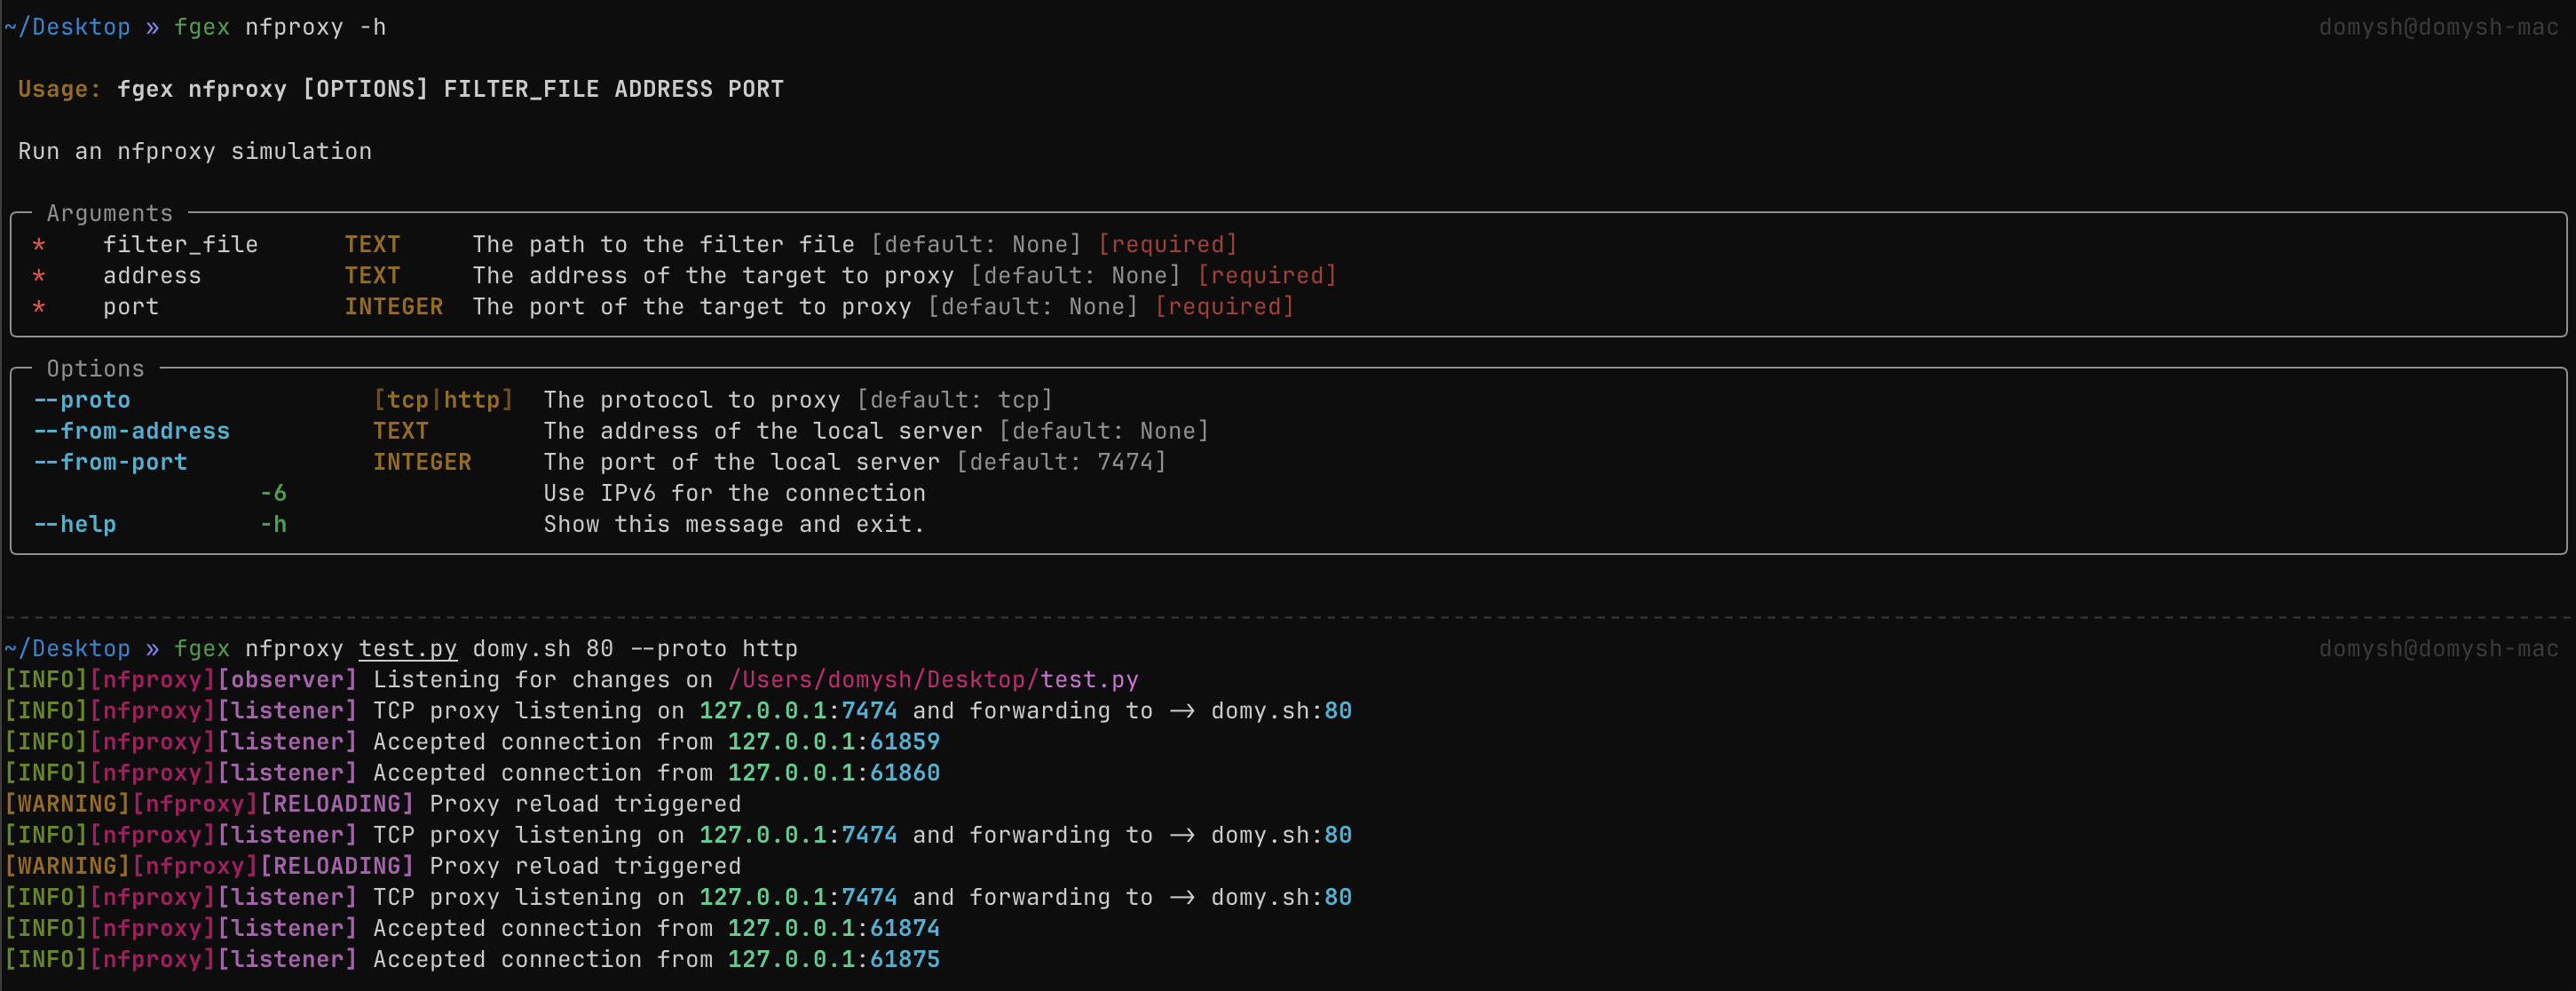
\includegraphics[width=0.98\textwidth]{images/chapter3/nfproxy_sim.png}
    \caption{Simulazione di nfproxy tramite il comando fgex}\label{fig:nfproxy_sim}
\end{figure}

